\Chapter{Téma elméleti kifejtése}
\label{Chap:tema}

\section {A mesterséges intelligencia}

\section{Kétszemélyes teljes információjú játékok}


\section{A Nim játék leírása}
A Nim játék egy kétszemélyes teljes információjú körökre osztott stratégiai játék. A játék egyszeregyből fakadóan számos változata, illetve továbbgondolása is létezik. Néhányat a későbbiekben röviden ismertetni is fogok. \\

A játék körökre bontott, azaz a játékosok felváltva teszik meg lépéseiket. A játék másik lényeges tulajdonsága, hogy teljes információjú játék, azaz a játék kezdetétől fogva mindkét játékos rendelkezésére áll az összes a játékra vonatkozó ismeret. Beleértve a szabályokat, és a teljes játékteret.\\

Nim játék esetében minden kör egy, és csakis egy lépésből áll, amit az éppen soron következő játékosnak kötelezően meg kell tennie. A játéktér tetszőleges számú halomból állhat, melynek elemeinek darabszáma csakugyan kötetlen (lehet egyforma, és akár mindegyik halom eltérő elemszámú). Hagyományosan ezek az elemek kavicsok, de igazából matematikai szempontból ezen entitások manifesztációja lényegtelen. Mindegyik lépés abból áll, hogy az éppen soron következő játékos az egyik nem üres elemszámú halomból elvesz legalább egy, legfeljebb az adott halom elemszámával megegyező darab (tehát akár az egész halmot) entitást a halomból.\\

A játék célja az, hogy amikor sorra kerülünk, akkor ne legyen már több halom, azaz az ellenfelet olyan helyzetbe hozzuk, hogy az végső lépést õ teszi meg, az utolsó entitás(okat) ő veszi el. Ez egyébként a leggyakrabban játszott Nim változat, Misère néven is ismert. Mint már említettem a Nim játéknak számos változata létezik, így előfordul, hogy fordítva játsszák, azaz nem az a soron következő játékos nyer, aki nem tud lépni, hanem az, aki a végső elem(eket) elveszi az utolsó halomból.\\


\section{A Nim játék története}
A Nim játék különböző variációit nagyon régóta játsszák. Pontos információink nincsenek, de egyes források arra engednek következtetni, hogy már az ókori Kínában is játszották ezt a játékot. Ugyancsak erre enged következtetni a \begin{CJK*}{UTF8}{gbsn}捡石子\end{CJK*}
(jiǎn-shízi) kínai eredetű játék, amely kísértetiesen hasonlít a Nim játékra, azzal a kivétellel, hogy ott egy halommal játsszák, igaz ennek is sok variánsa létezik, és az érvényes lépéseknek a szabályai bonyolultabbak. \\
Európában először a 16. század kezdetén tesznek róla említést, de igazán a figyelem középpontjába csak a 19. század végén került, amikor Charles L. Bouton tanulmányozta, majd 1901-ben a játék teljes elméletét kidolgozta. Úgy tudni a játékot is ő keresztelte el Nimnek, a német "Nimm" (elvenni) szó alapján. Más források arra hívják fel a figyelmet, hogy a "NIM" szót 180 fokkal elfordítva az angol "WIN" (nyerni) szót kaphatjuk meg. \\
A játék további ismertségre tett szert az 1939-es New York -i világkiállításon, ahol az 1886-ban alapított amerikai Westinghouse Electric Corporation cég bemutatta a Nimatront, egy olyan gépet, amely Nim játékot játszott. A dolog külön érdekessége, hogy ez volt világon az első elektronikus számítógépes játék.

\section{Ismertebb Nim variációk}
\subsection{Moore-Nim}
A Moore-Nim játék nevét kitalálójáról Eliakim Hastings Moore amerikai matematikusról kapta. Ez egyfajta általánosítása a több-halmos Nim játékoknak, ahol a játékosok egyszerre nem csak egy, hanem legalább egy, maximum $k$ halomból vehetnek el elemeket. Az elvehető elemek számát lehet korlátozni is.

\subsection{Póker-Nim}
A póker-Nimet egy előre rögzített számú entitással játsszák. Kezdetben az összes elemet felhasználva létrehoznak egy normál Nim játékot, majd a játékosok hagyományos Nim játékot játszanak azzal a különbséggel, hogy sorra kerülésükkor nem csupán elvehetnek a halomból, hanem már az elvett elemeket újra felhasználva a halomhoz hozzáadjanak elemeket. \\
Könnyen belátható, hogy új elemek hozzáadása a halomhoz nem befolyásolja lényegesen a játékmenetet, hiszen a következő játékos tetszőleges számú elemet elvehet egy kupacból beleértve az előző játékos által hozzáadott extra elemeket.

\subsection{Lasker-Nim}
Nevét az Német-amerikai sakk és Go mesterről Edward Laskerről kapta. Ő javasolta, hogy a hagyományos Nim játékot egészítsék ki egy új érvényes művelettel, a halmok kettébontásával. Ez a kettébontás nem feltétlenül két egyenlő félre való bontást jelent, a két új halom elemszámainak arányára vonatkozóan nincsen megkötés.

\subsection{End-Nim}
End-Nim esetében a halmok sorba vannak rendezve, és bár a játékosok a hagyományos Nim szabályai szerint játszanak, azonban csupán a sor két végén levő halmokból vehetnek el elemeket.

\subsection{Fibonacci-Nim}
Ezt a Nim variánst egyetlen halommal játsszák, de a benne lévő elemek számára nincsen megkötés. A hagyományos Nim játékhoz képest az a különbség, hogy a játékosok legfeljebb mindig az előző játékos által elvett elemek kétszeresét veheti el. A kezdő lépést megtevő játékos tetszőleges (de nem az összes) elemet elvehet a halomból. Az utolsó elemet elvevő játékos nyer.

\subsection{Wythoff-Nim}
Willem Abraham Wythoff Holland matematikusról kapta a nevét, aki 1907-ben publikálta a játék matematikai analízisét. A játékot két érmehalommal játsszák, minden körben a soron lévő játékosnak el kell vennie valamennyi érmét az egyik kupacból, vagy mindkét halomból egyenlő számú érmét. Az nyer, aki az utolsó érmét, vagy érméket elveszi. \\
A játék megegyezik a királynőt a sarokba játékkal, ahol egy vezért kell eljuttatni valamelyik (általában bal alsó) sarokba, de egy lépés csak akkor érvényes ha azzal közelebb kerül a célhoz.

\subsection{End-Wythoff}
Az egyik legbonyolultabb Nim játék. Ez ötvözi az End-Nim, és a Wythoff-Nim szabályait. Tetszőleges számú halommal játsszák, de a halmok sorba vannak rendezve, és a soron következő játékos csak a szélén lévő halomból vehet el elemeket, vagy a szélén lévő két kupacból megegyező számú elemet.

\subsection{Az osztó játék}
Egy tetszőleges természetes számról indulva a játékosok minden körben elosztják ezt a számot egy olyan prím szám valamely hatványával, amely osztója az éppen aktuális számnak (kivéve természetesen az 1). Az a játékos, amelyik a végén eljut az 1-re, az nyer, vagy veszít attól függően melyik változatát játsszák.

\subsection{A kivonó játék}
Sokan tévesen ezt a variánst ismerik Nim játékként. Többnyire egy halommal játsszák, azonban az elvehető elemek maximális számára van valamilyen $S(1, 2, ..., k)$ korlát.

\subsection{A 21 játék}
Ezt a játékot Misère játékként játsszák. A kezdő mond egy 20-nál kisebb pozitív egész számot, majd a soron következő játékosok a számot 1, 2, 3-mal növelhetik, de nem léphetik át a 21-et. Az a játékos, amelyik a 21 kimondására kényszerül elveszíti a játszmát.

\subsection{A 100 játék}
A 21 játékhoz nagyon hasonló. Itt a célszám 100, és az azt elérő játékos nyer. A kezdőszám a 0, és a játékosok körönként 1 és 10 közötti egész számot adhatnak hozzá az aktuális értékhez.

\subsection{Körkörös Nim (Kayles)}
Az elemek ebben a variánsban körben helyezkednek el, és a soron következő játékos legfeljebb $k$ egymást követő elemet vehet el a körből. Játszható normál és Misère változatban is.

\subsection{Grundy játéka}
A Grundy játéka egy halommal indul benne tetszőleges számú elemmel. A hagyományos Nim játéktól eltérően itt nem elemeket vesznek el a halomból, hanem a halmokat bontják két nem egyforma méretű halomra. A játéknak akkor van vége, amikor már nincs olyan halom, amit ketté lehetne bontani két nem egyforma méretű halommá. Ezt a variánst is lehet normál, illetve Misère módon játszani.

\subsection{Mohó Nim}
Normális, és Misère módon is játszható a Mohó-Nim, ami csupán annyiban különbözik a hagyományos Nim játéktól, hogy a játékosok csak a legnagyobb elemszámú halomból vehetnek el elemeket.

\subsection{Építő Nim}
Az építő-Nim két részből tevődik össze. Először felépítik Nim játékot az előre megadott számú elemet felhasználva, majd azt lejátsszák. Felépítéskor a játékosok körönként 1-1 elemet raknak (a kezdetben üres) előre meghatározott számú halomba.

\subsection{Northcott-sakk}
A Northcott-sakk egy 8x8-as sakktáblából áll. Kezdetben a játékosok (egymás elől elrejtve) elhelyezik a bábuikat (mindegyik oszlopba csak egyet téve) a saját térfelükön. Miután ezzel végeztek elkezdődik a játék. A játékosok felváltva lépnek, minden körben csak az egyik saját bábujukkal csak előre, és legfeljebb annyit amennyi üres hely van az ő bábuja, és az ellenfél bábuja között, azaz az ellenfél bábuját nem ütheti le, és nem ugorhatja át.\\

\begin{figure}[h]
	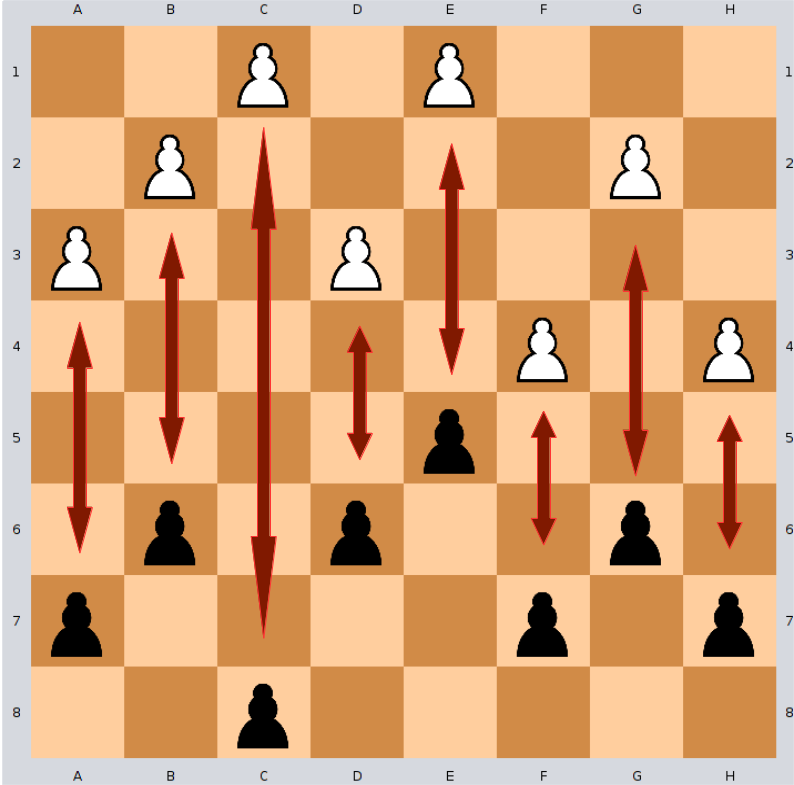
\includegraphics[width=8cm, height=8cm]{northcott-chess}
	\centering
	\caption{Nortcott-sakk táblája. A nyilak a bábuk közti távolságot jelöli, ami a halom méretének felel meg.}
\end{figure}

Ha jobban belegondolunk ez a játék egy az egyben megfeleltethető a hagyományos Nim játéknak, ebből következően játszható sima, és Misère módon is.\\ 
Szempontunkból ez a variáns azért is különösen érdekes, mert a szakdolgozatom tartalmazza ennek a játéknak a példaimplementációját, ami ráadásul ténylegesen Nim játékot játszik a háttérben ugyan azt a játékosztályt használva ezzel szemléltetve, hogy mennyire is visszavezethető a Northcott-sakk a standard Nim játékra.

\section{A Nim játék matematikai háttere}


\section{Nyerő stratégia}
Jelen dolgozat írása közben sok érdekes, és informatív internetes oldallal találkoztam. A {\em \url{ https://brilliant.org/wiki/nim/}} oldalon találtam a nyerő stratégiához egy remek leírást bizonyítással egybekötve, amihez úgy érzem nem tudnék érdemben hozzá tenni, ugyanakkor ez a dolgozat bizonyítás nélkül nem lehet teljes, így az alábbiakban közlöm ezen oldalon található angol nyelvű nyerő stratégiájának leírását, illetve annak bizonyításának bizonyítás magyar fordítását. Az eredeti bizonyítás Charles L. Boutontól származik, aki elsőként dolgozta ki a Nim játék teljes matematikai hátterét. (Lásd irodalomjegyzék) \\ \\

A nyerő stratégia bemutatását kezdjük egy nagyon fontos definícióval:
\begin{definition}
	Az $a$ és $b$ nemnegatív egész számokon elvégzett $a \oplus b$ műveletet nim-összegnek nevezzük, amennyiben a következő módon kerül kiszámításra. Jelentse $a$ és $b$ kettő különálló hatványainak összegét. Vessük el kettő olyan hatványait, amelyek többször is szerepelnek, majd a fennmaradó hatványokat adjuk össze.
\end{definition}

\begin{remark}
	A nim-összeg gyakorlatilag a XOR logikai műveletnek felel meg, implementálás során is ezt használtam fel.
\end{remark}

Például $3 \oplus 5$ a következőképpen számítható ki. A $3 = 2^1 + 2^0$, és az $5 = 2^2 + 2^0$. Mivel a $2^0$ kétszer szerepel, ezért eldobjuk, a maradékot pedig  összeadjuk $2^1 + 2^2$ kiadva az $3 \oplus 5 = 6$ eredményt. \\

Bizonyítható, hogy $\oplus$ asszociatív, ezáltal több szám nim-összegét $a_1 \oplus a_2 \oplus ... \oplus a_n$ definiálja. \\

Legyen egy adott normál Nim állás (a halmok méretei) $a_1, a_2, ... a_n$, az éppen lépő játékos akkor nyer, ha $a_1 \oplus a_2 \oplus ... \oplus a_n \neq 0$; és a nyerő lépést a $i \in \{1, 2, .., n\}$ meghatározásával lehet megtalálni, és a $b_i \in \{0, 1, ..., a_i -1\}$ amivel tehát $a_1 \oplus a_2 \oplus ... \oplus a_{i-1} \oplus b_i \oplus a_{i+1} + a_{i+2} \oplus ... \oplus a_n = 0$ elvéve valamennyi elemet az $i$ halmazból $b_i$ elemet hátrahagyva. Ha $a_1 \oplus a_2 \oplus ... \oplus a_n = 0$, akkor az éppen lépő játékos veszít. \\

Misère Nim esetében a stratégia majdnem teljesen azonos. Egészen addig, amíg a javasolt lépés elvégzése után marad legalább egy halom 2, vagy több elemmel használjuk a normál Nim stratégiáját. Amennyiben a javasolt lépés után nem marad legalább egy halom kettő, vagy több elemmel más lépést kell tennünk:
\begin{itemize}
	\item Ha a javasolt lépés után 1 elem maradna hátra, akkor vegyük el az egész halmot, vagy
	\item Ha a javasolt lépés után nem maradna elem a halomban, úgy hagyjunk benne egy elemet.
\end{itemize}
Más szóval a helyes lépés az, hogy páratlan számú halmokat hagyjunk meg 1 elemmérettel. (Normál esetben páros számú 1 méretű halmokra törekszünk, ezzel a nim-összeget zérussá téve) 


\subsection{Nyerő stratégia bizonyítása}
\begin{theorem}
	A soron következő játékos akkor, és csak akkor nyeri meg a normál Nim játékot, ha a halmok nim-összege nem zérus
\end{theorem}

\begin{proof}
Kezdésnek vegyük az egyszerű alapesetet: ha mindegyik halom elemszáma zérus, akkor a soron következő játékos veszít, és a nim-összeg is zérus. Ettől fogva tegyük fel, hogy nem mindegyik halom üres. \\

Először is vegyük észre, hogy a nim-összeg számos fontos tulajdonsággal rendelkezik. Minden nem negatív a, b, c egész számra igaz, hogy:
\begin{itemize}
	\item Asszociatív: $(a \oplus b) \oplus c = a \oplus (b \oplus c)$
	\item Kommutatív: $a \oplus b = b \oplus a$
	\item Létezik semleges eleme: $0 \oplus a = a$
	\item Öninverz: $a \oplus a = 0$
	\item Lehetséges egyszerre több több számnak a Nim-összegét meghatározni oly módon, hogy felírjuk az összes számot 2 különálló hatványaira, majd megkeressük 2 összes olyan hatványát, mely páratlanszor szerepel, végül összeadjuk ezeket 2 hatványokat úgy, hogy mindegyiket csak egyszer vesszük. Például: \\
	$1 \oplus 3 \oplus 7 = (2^0) \oplus (2^0 + 2^1) \oplus (2^0 + 2^1 + 2^2) = 2^0 + 2^2 = 5$
\end{itemize}

Tegyük fel, hogy a halmok elemszáma minden lépés előtt $a_1, a_2, ..., a_n$, illetve $b_1, b_2, ..., b_n$ minden lépés végén. Feltételezzük továbbá, hogy amennyiben $k$ halmon végzünk el egy lépést, akkor minden $i \neq k$ -ra $a_i = b_i$. Legyen $s = a_1 \oplus a_2 \oplus ... \oplus a_n$ és $t_n = b_1 \oplus b_2 \oplus ... \oplus b_n$. Ekkor a következőket kapjuk:
\begin{alignat*}{1}
	t &= 0 \oplus t \\
	&= (s \oplus s) \oplus t \\
	&= s \oplus (s \oplus t) \\
	&= s \oplus ((a_1 \oplus a_2 \oplus ... \oplus a_n) \oplus (b_1 \oplus b_2 \oplus ... \oplus b_n)) \\
	&= s \oplus ((a_1 \oplus b_1) \oplus (a2_ \oplus b_2) \oplus ... \oplus (a_n \oplus b_n)) \\
	&= s \oplus (0 \oplus 0 \oplus ... \oplus 0 \oplus (a_k \oplus b_k) \oplus 0 \oplus ... \oplus 0) \\
	&= s \oplus (a_k \oplus b_k).
\end{alignat*}
Most két eset bizonyítása következik. \\

\textbf{Első eset:} Ha $s = 0$, akkor $t \neq 0$. Amennyiben az eredeti méretek nim-összege zérus, úgy a lépést végző játékos vesztésre áll (ebből kifolyólag a nim-összeget nem-zérussá kell alakítania)\\
Azt állítjuk, hogy $a_k \oplus b_k \neq 0$. Tegyük fel, hogy így is van, ekkor:

\begin{alignat*}{2}
	a_k &= a_k \oplus 0 \\
	&= a_k \oplus (a_k \oplus b_k) \\
	&= (a_k \oplus a_k) \oplus b_k \\
	&= b_k.
\end{alignat*}

Tehát $a_k = b_k$. De ez ellent mond annak a ténynek, hogy a lépést végrehajtó játékos a $b_k$ halmon végezte el a lépést, s így nem is csökkentette a halom méretét. \\ \\
Tehát mivel $a_k \oplus b_k \neq 0$, így:

\begin{alignat*}{3}
	t &= a \oplus (a_k \oplus b_k) \\
	&= 0 \oplus (a_k \oplus b_k) \\
	&= a_k \oplus b_k \\
	&\neq 0.
\end{alignat*}

\textbf{Második eset:} Ha $s \neq 0$, akkor lehetséges, hogy $t = 0$. Amennyiben  az eredeti halmok nim-összege nem zérus, abban az esetben az éppen lépő játékos nyertes helyzetben van. (hiszen a nim-összeget zérussá tudja alakítani) \\

Vegyük számításba, hogy 2 legmagasabb hatványa $2^k$ nem nagyobb, mint s. Léteznie kell legalább egy olyan $a_i$-nak, ami szintén tartalmazza $2^k$-t, különben $2^k$ nem szerepelhetne s-ben. Most vegyük $b_i = s \oplus a_i$-t. A $b_i$ értéke $2^k$-nal csökken, és legfeljebb $2^{k-1} + 2^{k-2} + ... + 2^0 = 2^k -1 $-gyel nő. (2 minden visszamaradt hatványa kiadja s-t, hozzáadódva az értékhez; például $s = s^2 + 2^1 + 2^0$ és $a_i = 2^3 + 2^2$ kiadja $b_i = 2^3 + 2^1 + 2^0$-t), tehát $b_i < a_i$. Továbbá:
\begin{alignat*}{1}
	t &= s \oplus (a_i \oplus b_i) \\
	&= s \oplus (a_i \oplus (s \oplus a_i)) \\
	&= (s \oplus s) \oplus (a_i \oplus a_i) \\
	&= 0.
\end{alignat*}

Ezzel a tétel bizonyítva van.
\end{proof}

